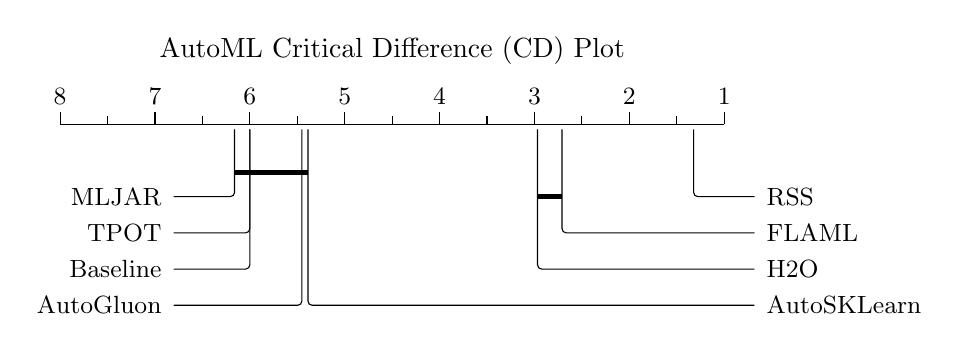
\begin{tikzpicture}[
  treatment line/.style={rounded corners=1.5pt, line cap=round, shorten >=1pt},
  treatment label/.style={font=\small},
  group line/.style={ultra thick},
]

\begin{axis}[
  clip={false},
  axis x line={center},
  axis y line={none},
  axis line style={-},
  xmin={1},
  ymax={0},
  scale only axis={true},
  width={\axisdefaultwidth},
  ticklabel style={anchor=south, yshift=1.3*\pgfkeysvalueof{/pgfplots/major tick length}, font=\small},
  every tick/.style={draw=black},
  major tick style={yshift=.5*\pgfkeysvalueof{/pgfplots/major tick length}},
  minor tick style={yshift=.5*\pgfkeysvalueof{/pgfplots/minor tick length}},
  title style={yshift=\baselineskip},
  xmax={8},
  ymin={-5.5},
  height={6\baselineskip},
  xtick={1,2,3,4,5,6,7,8},
  minor x tick num={1},
  x dir={reverse},
  title={AutoML Critical Difference (CD) Plot},
]

\draw[treatment line] ([yshift=-2pt] axis cs:1.3225806451612903, 0) |- (axis cs:0.6559139784946236, -2.0)
  node[treatment label, anchor=west] {RSS};
\draw[treatment line] ([yshift=-2pt] axis cs:2.7096774193548385, 0) |- (axis cs:0.6559139784946236, -3.0)
  node[treatment label, anchor=west] {FLAML};
\draw[treatment line] ([yshift=-2pt] axis cs:2.967741935483871, 0) |- (axis cs:0.6559139784946236, -4.0)
  node[treatment label, anchor=west] {H2O};
\draw[treatment line] ([yshift=-2pt] axis cs:5.387096774193548, 0) |- (axis cs:0.6559139784946236, -5.0)
  node[treatment label, anchor=west] {AutoSKLearn};
\draw[treatment line] ([yshift=-2pt] axis cs:5.451612903225806, 0) |- (axis cs:6.827956989247312, -5.0)
  node[treatment label, anchor=east] {AutoGluon};
\draw[treatment line] ([yshift=-2pt] axis cs:6.0, 0) |- (axis cs:6.827956989247312, -4.0)
  node[treatment label, anchor=east] {Baseline};
\draw[treatment line] ([yshift=-2pt] axis cs:6.0, 0) |- (axis cs:6.827956989247312, -3.0)
  node[treatment label, anchor=east] {TPOT};
\draw[treatment line] ([yshift=-2pt] axis cs:6.161290322580645, 0) |- (axis cs:6.827956989247312, -2.0)
  node[treatment label, anchor=east] {MLJAR};
\draw[group line] (axis cs:5.387096774193548, -1.3333333333333333) -- (axis cs:6.161290322580645, -1.3333333333333333);
\draw[group line] (axis cs:2.7096774193548385, -2.0) -- (axis cs:2.967741935483871, -2.0);

\end{axis}
\end{tikzpicture}